\externaldocument{chapter4}
\externaldocument{chapter1}
\externaldocument{chapter5}
\chapter{Literature Survey and Model Selection } % Main chapter title

\label{Chapter3} % For referencing the chapter elsewhere, use \ref{Chapter2} 

Using content-based music information for solving several music information retrieval tasks is not new, but a decade long research efforts have been put. In section \ref{literature}, the dynamics of the literature that has lead to the use of deep learning techniques for MIR tasks have been discussed. In the previous chapter, the abstract algorithm for music classification task was introduced. However, it can be seen that there are plenty of parameters (like sampling rate, STFT parameters, CNN hyper-parameters) to fix. Therefore, in this chapter, we also briefly dive into some of the successful algorithms in the literature to demonstrate the optimal choice parameters or network settings one can use. In section \ref{model}, the inferences from state of art techniques have been used to short list models for the experiments.       


\section{Literature Review}
\label{literature}
Dedicated analysis for music features emerged due to the fact that music signals possess specific acoustic and structural characteristics that distinguish them from spoken language or other non musical signals. In the previous chapter, computing the optimal features for a context-based classification task using deep learning was formalised. However, it is not always true that such \textit{learned} features will perform better than \textit{hand-crafted} features. The underlying issue is ultimately one of \textit{organization} and \textit{variance} of the features. 
\bigskip 

\noindent \textit{\textbf{Feature organization :}} The better organized a feature is to answer some question, the simpler it is to assign or infer semantic meaning. Thus a feature representation should explicitly reflect a desired semantic organization. 

\noindent \textit{\textbf{Feature variance :}} A feature representation is said to be \textit{noisy} when variance in the data is misleading or uninformative, and \textit{robust} when it predictably encodes these invariant attributes. Complicated classifying methods are necessary only to compensate for any noise and hence a \textit{robust} feature representation is important.
\bigskip

\noindent In the following subsections, adoption of feature learning techniques for multi-label classification task are elaborated. All the models (except \cite{MusicMotive}) were experimented for \textit{multi-label classification task} on Magna Tag a Tune dataset(MTT)\cite{MTT} with about 29K clips which are 29.1s long.

\subsection{From hand-crafting to feature learning}
\label{featurelearning}
A number of features have been engineered in the past that are relevant for different MIR tasks. MFCC features (ref. \ref{mfcc}), originally developed for speech recognition task often proved efficient for genre classification and tagging. At the same time, some machine learning algorithms were also used to adopt feature learning on spectrogram frames. Results from some proceedings that compare MFCCs (feature engineering) with feature learning for \textit{multi-label classification task} have been discussed.
\bigskip

\noindent \textbf{Temporal pooling and multiscale learning for automatic annotation and ranking of music audio. 2011 \cite{featurelearn1}:}\\
\\
\noindent The pipe line of their algorithm is shown below. The formalism of the notations used are consistent with explanations in chapter 2. The PCA whitened mel-power spectrogram (ref. \ref{pca}) (unsupervised learning for frame features) is compared with MFCC features (engineered features) on Magna tag a tune dataset. It was shown that the former achieve a performance of \textbf{AUC 0.87} out performing MFCCs which was 0.77. From this research, we can infer that unsupervised learning can extract features more relevant than MFCCs for music tagging.  
\bigskip

\noindent \textbf{\textit{Parameter settings :}} Signal ($\textbf{a}$) is sampled at 22.1 KHz. Then STFT with window length 1024 and stride 512 is computed with FFT algorithm (ref. \ref{stft}). This is followed by conversion to mel power-spectrogram with 128 bins, followed by PCA Whitening which selects the top 120 variant frequencies. The resulting reduction is transformed by the operator $\textbf{W}_{L1}$ that learns (supervised) optimal features for some pooling function $T_{(POOL)}$. The temporal pooling is done by summarizing every 2.3s frame with suitable functions (see \cite{featurelearn1} for details). The resulting feature is then classified by two layer perceptron with 1000 hidden units with sigmoid ($\sigma$) activations. This algorithm is also an illustration for how supervised feature learning is pushed beyond the classifier and into the temporal pooler, but not into the frame-wise reduction stage (see chapter 2 \ref{training}).

\begin{algorithm}
  \caption{$\textbf{pred}$ = MODEL($\textbf{a}$) }\label{Temporal Pooling}
  \begin{algorithmic}[1]
    \Statex \textbf{Input :} $\textbf{a} \in \mathbb{R}^{N}$
    \Statex \textbf{Output :} $\textbf{pred}$ \Comment{indices of predicted labels} 
    \State $\textbf{C} = \textbf{a} \star \textbf{W}_{STFT}$ \Comment{$\textbf{C} \in \mathbb{C}^{M \times P}$}
    \State $\textbf{C} \leftarrow \textbf{C} \odot \textbf{C}$ 
    \State $\textbf{X} = \textbf{C} \star \textbf{W}_{MEL}$ \Comment{$\textbf{X} \in \mathbb{R}^{128 \times P}$}
    \State $\textbf{Y}_{1} = D_{(PCAW)}(\textbf{X})$ \Comment{$\textbf{Y}_{1} \in \mathbb{R}^{120 \times P}$}
    \State $\textbf{Y}_{2} = \textbf{W}_{L1}\textbf{Y}_{1}$  \Comment{$\textbf{W}_{L1} \in \mathbb{R}^{S \times 120}, \textbf{Y}_{2} \in \mathbb{R}^{T \times P}$}
    \State $\textbf{f} = T_{(POOL)}(\textbf{Y}_{2})$ \Comment{$\textbf{f} \in \mathbb{R}^{T.W}$}
    \State $\bm{\zeta} = \sigma(\textbf{W}_{L3}\sigma(\textbf{W}_{L2}\textbf{f}))$ \Comment{$\textbf{W}_{L2} \in \mathbb{R}^{1000 \times T.W}, \textbf{W}_{L3} \in \mathbb{R}^{L \times 1000}$}
    \State $\textbf{pred} = \{ b(\zeta_{i}) | b(\zeta_{i}) = 1 \}$ \Comment{$ i \in \{1,2,..,L\}, b( \zeta_{i}) \in \{0,1\}$}
  \end{algorithmic}
\end{algorithm}
\FloatBarrier
\bigskip

\noindent \textbf{Multiscale Approaches To Music Audio Feature Learning. 2012\cite{MultiScale}:}\\
\\
\noindent The result reported by this model is the current state-of-art on MTT dataset (\textbf{AUC 0.898}). In this research, supervision is introduced only in the classifier. The reduction and temporal approximation are done with sophisticated unsupervised learning. Here the mel-spectrogram is transformed to $W$ \textit{gaussian pyramids} and features from each level of the pyramid are extracted separately and concatenated. At each level, the spectrogram is divided into T segments and Bag of Frames features are extracted separately on every segment after PCA whitening operation. The signal is sampled at 16 KHz and the STFT window size is 1024 and hop size 512. The mel-spectrogram has 200 bins. 
\begin{algorithm}
  \caption{$\textbf{pred}$ = MODEL($\textbf{a}$) }\label{multiscale}
  \begin{algorithmic}[1]
    \Statex \textbf{Input :} $\textbf{a} \in \mathbb{R}^{N}$
    \Statex \textbf{Output :} $\textbf{pred}$ \Comment{indices of predicted labels} 
    \State $\textbf{C} = \textbf{a} \star \textbf{W}_{STFT}$ \Comment{$\textbf{C} \in \mathbb{C}^{M \times P}$}
    \State $\textbf{C} \leftarrow \textbf{C} \odot \textbf{C}$ 
    \State $\textbf{X} = \textbf{C} \star \textbf{W}_{MEL}$ \Comment{$\textbf{X} \in \mathbb{R}^{R \times P}$}
    \For{$i \in \{1,..,Z\}$}
     \State $\textbf{Y} \leftarrow Gaussian\_Pyramid(\textbf{X},i)$ \Comment{$\textbf{Y} \in \mathbb{R}^{R \times W1_{i}}$}
     \For{$j \in \{1,...,T\}$}
       \State $\textbf{F}_{1}[:,j] \leftarrow BagOfFrames(D_{(PCAW)}(\textbf{Y}_{1}))$ \Comment{$\textbf{F}_{1} \in \mathbb{R}^{T \times W_{i}}$}
      \EndFor
    \State $\textbf{F}[i] \leftarrow T_{MaxPool}(\textbf{F}_{1})$ \Comment{$\textbf{F} \in \mathbb{R}^{T \times W}$}
    \EndFor
    \State $\textbf{f} = Flatten(\textbf{F})$ \Comment{$\textbf{f} \in \mathbb{R}^{T.W}$}
    \State $\bm{\zeta} = \sigma(\textbf{W}_{L3})ReLU(\textbf{W}_{L2}\textbf{f}))$ \Comment{$\textbf{W}_{L2} \in \mathbb{R}^{1000 \times T.W}, \textbf{W}_{L3} \in \mathbb{R}^{L \times 1000}$}
    \State $\textbf{pred} = \{ b(\zeta_{i}) | b(\zeta_{i}) = 1 \}$ \Comment{$ i \in \{1,2,..,L\}, b( \zeta_{i}) \in \{0,1\}$}
  \end{algorithmic}
\end{algorithm}
\FloatBarrier

\subsection{Transfer Learning by supervised pre-training}
\label{transfer}
Supervised feature learning techniques  typically require large amounts of training data to work well. But sometimes, features learned on large datasets can be used for other datasets, either as a \textit{black-box} extractor (feature extractor is not further trained on target dataset) or as a \textit{fine-tuned} feature extractor (feature extractor is further trained after initializing weights). To do this, it is essential to have a source task that requires a very rich feature representation, so as to ensure that the information content of this representation is likely to be useful for other tasks
\bigskip

\noindent \textbf{Transfer learning by supervised pre-training for audio-based music classification. 2014\cite{TransferLearning}:}\\
\\
In this research, the reduction operators trained on MSD dataset (~1000K clips) are used as \textit{black-box} feature extractor while training on MTT dataset and the resulting classification performance still achieved \textbf{AUC 0.88} outperforming baseline MFCC. The workflow for source and target are shown below,
\begin{figure}[h] 
\centering
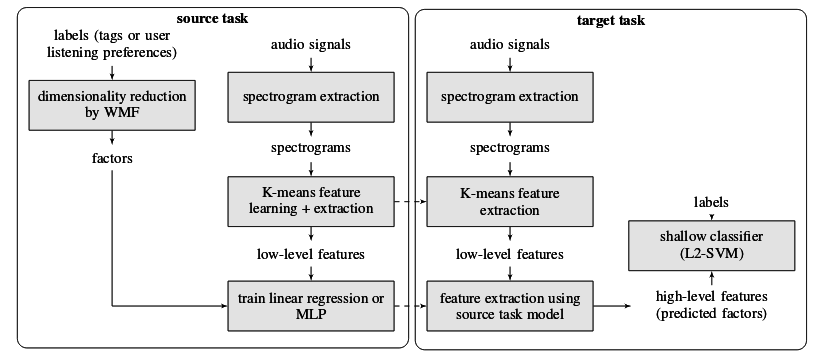
\includegraphics[width=0.95\textwidth]{specLeak1}
\caption{Schematic overview of the workflow of transfer learning\cite{TransferLearning}}
 \label{fig:transfer learning}
 \end{figure}
\FloatBarrier
\bigskip

\noindent \textbf{Source task}: 
The features from audio spectrograms are learned through unsupervised learning by spherical K-Means. A multi layer perceptron (supervised) is then stacked to obtain final prediction. So the output from the penultimate layer of MLP are treated as transferable features. To tackle problems created by redundant and sparse labels, dimensionality reduction is done in the label space using Weighted Matrix Factorization (WMF). The model is then trained to predict the reduced label representation.
\bigskip

\noindent \textbf{Target task}
Next,  the trained models are used to extract features from other datasets, which are then passed to train shallow classifiers for different but related target tasks. This workflow is visualized in figure \ref{fig:transfer learning}. Dashed arrows indicate transfer of the learned feature extractors from the source task to the target task.
\bigskip


\subsection{Convolutional Neural Networks}
\label{convolution}
It was shown that supervised learning can be pushed deep into the feature extraction pipeline by stacking multiple layers of learnable convolution filters (ref. \ref{stacked}). The idea was to replace the application specific dimension reductions with Convolution Neural Networks(CNN). In this section, some works that throw insights into CNN architecture settings are discussed. 
\bigskip

\noindent \textbf{End-to-end learning for music audio. 2014\cite{EndToEnd}:}\\
\\
\noindent As shown in chapter 2, all operations including FFT can be defined in terms of convolutions. In this research, they investigate whether it is possible to push supervision directly on to raw audio signal. The signal was convolved with 3 layers of 1D convolutions followed by two layer perceptron. Thus, feature learning is applied directly on the input and this is called\textit{ end to end learning}. They compared the \textit{end to end learning} approach with supervised learning after mel-power-spectrogram on MTT dataset (i.e, retaining $\textbf{W}_{STFT}$ and $\textbf{W}_{MEL}$). It was found that, discarding STFT hurt the performance. CNN from mel-spectrogram achieved \textbf{AUC 0.8815}, but on including supervision directly on audio signal, AUC dropped to 0.8487.     
 
\begin{minipage}[t]{7.5cm}
  \vspace{0pt}  
  \begin{algorithm}[H]
    \caption{CNN(raw audio) [\textbf{0.84}]}\label{alg:endtoend}
    \begin{algorithmic}[1]
      \Statex \textbf{Input :} $\textbf{a} \in \mathbb{R}^{N}$
      \Statex \textbf{Output :} $\textbf{pred}$ 
      \State $\textbf{Y}_{1}  = \bm{\Phi_{1}}(\textbf{a}\star{\textbf{W}_{C1}}^{(256)})$
      \State $\textbf{Y}_{2} =  MaxPool(ReLU(\textbf{Y}_{1}\star{\textbf{W}_{C2}}^{(1)}))$
       \State $\textbf{Y}_{3} = MaxPool(ReLU(\textbf{Y}_{2}\star{\textbf{W}_{C3}}^{(1)}))$
       \State $\textbf{f} = Flatten(\textbf{Y}_{3})$
       \State $\bm{\zeta} = \sigma(\textbf{W}_{L2}ReLU(\textbf{W}_{L1}\textbf{f}))$
       \State $\textbf{pred} = \{ b(\zeta_{i}) | b(\zeta_{i}) = 1 \}$ \Comment{$ i \in \{1,2,..,L\}, b( \zeta_{i}) \in \{0,1\}$}
       \State
   \end{algorithmic}
  \end{algorithm}
\end{minipage}%
\begin{minipage}[t]{7.5cm}
  \vspace{0pt}
  \begin{algorithm}[H]
    \caption{CNN(Mel-Power-Spectrogram) [\textbf{0.88}]}\label{alg:meltoend}
     \begin{algorithmic}[1]
      \Statex \textbf{Input :} $\textbf{a} \in \mathbb{R}^{N}$
      \Statex \textbf{Output :} $\textbf{pred}$ \Comment{indices of predicted labels} 
      \State $\textbf{C}  = \textbf{a} \star \textbf{W}_{STFT}$
      \State $\textbf{C}  \leftarrow \textbf{C} \odot \textbf{C}$
       \State $\textbf{X} = \textbf{C} \star \textbf{W}_{MEL}$
       \State $\textbf{Y}_{1} =  MaxPool(ReLU(\textbf{X}\star{\textbf{W}_{C1}}^{(1)}))$
       \State $\textbf{Y}_{2} = MaxPool(ReLU(\textbf{Y}_{1}\star{\textbf{W}_{C2}}^{(1)}))$
       \State $\textbf{f} = Flatten(\textbf{Y}_{2})$
       \State $\bm{\zeta} = \sigma(\textbf{W}_{L2}ReLU(\textbf{W}_{L1}\textbf{f}))$
       \State $\textbf{pred} = \{ b(\zeta_{i}) | b(\zeta_{i}) = 1 \}$
   \end{algorithmic}
  \end{algorithm}
\end{minipage}
\FloatBarrier
\noindent Algorithm \ref{alg:endtoend} is an the end-to-end learned classifier. The signal $\textbf{a}$ is convolved with filter $\textbf{W}_{C1}$ by replacing the STFT operation. Function $\bm{\Phi}_{1}$ is an element-wise logarithmic compression refereed in \cite{EndToEnd}.  Two more layers of CNN are stacked over. The non-linearities in the second and third layer are $ReLU$ (see Sec. \ref{issues}) followed by a pooling operation ($MaxPool$). Max pooling is done by segmenting the resulting reduction and taking just the maximum value in each segment. This is done to further reduce the dimension. The features from CNN are taken by the classifier. This model expects input of fixed size (29.1s) and hence a temporal approximator is not used. During test-run, predictions for an arbitrary length of signal is done by segmenting it to 29.1s sections are performing classification separately on each section.  
\bigskip

\noindent \textbf{Experimenting with musically motivated convolutional neural networks. 2016\cite{MusicMotive}:}\\
\\
\noindent In the previous section, only 1D convolution with filter sizes directly motivated by hand-crafted methods were tested for comparison. But usually, the convolution operation allows flexibility in choosing the filter sizes. In this research, the authors discuss how convolution filters with different shapes can fit specific musical concepts. 
\begin{figure}[h]
       \begin{subfigure}[b]{0.3\textwidth}
        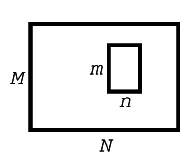
\includegraphics[width=\textwidth]{square}
        \caption{Rectangular filter }
        \label{fig:square}
       \end{subfigure}
	    \begin{subfigure}[b]{0.3\textwidth}
        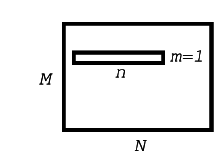
\includegraphics[width=\textwidth]{time}
        \caption{
        Time filter
        }
        \label{fig:time}
       \end{subfigure}
       	    \begin{subfigure}[b]{0.3\textwidth}
        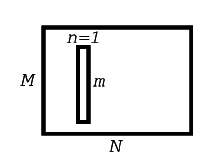
\includegraphics[width=\textwidth]{freq}
        \caption{
        Frequency filter
        }
        \label{fig:freq}
       \end{subfigure}
       \caption{Different Filter sizes\cite{MusicMotive}}\label{fig:STFT}
\end{figure}
\FloatBarrier
\bigskip 
\noindent \textit{Time filters} (fig \ref{fig:time}) can learn temporal cues like \textit{onset} and \textit{beats per minute}, while \textit{frequency filters} (fig \ref{fig:freq}) can differentiate timbre and note. \textit{Rectangular filters} can learn short time sub-bands (Bass, kick, drums)\cite{MusicMotive}. It was shown in their experiments that \textit{rectangular filters} or combination of time and frequency filters performed better than using just time or frequency filter. These experiments were done for a genre classification task. 
\bigskip
 
\noindent \textbf{Automatic tagging using deep convolutional neural networks. 2016\cite{choi_cnn}:}\\
\\
\noindent With several choices for filter sizes, number of filters and number of layers, there are myriads of CNN  architecture choices. The proposed architecture in this research achieves close to state of art performance on MTT dataset (\textbf{0.894 AUC}). The audio samples were down-sampled to 12 KHz and supervision was pushed until mel spectrogram extraction (with 96 bins). They also compared the features - MFCCs, CNN over STFT and CNN over Mel-log power spectrogram and report that the latter performs significantly better. 
\begin{table}[H]
\centering
    \begin{tabular}{ | p{5cm} | l |}
    \hline
    \textbf{Features} & \textbf{AUC} \\ \hline
    STFT $\rightarrow$ CNN &  0.846\\ \hline
    STFT $\rightarrow$ MEL $\rightarrow$ CNN &  \textbf{0.894}\\ \hline
    STFT $\rightarrow$ MEL $\rightarrow$ MFCC &  0.862 \\ \hline
    \hline
    \end{tabular}
\caption{Comparision of features}
\end{table}
    
\noindent To exploit the advantage of PCA Whitening proven in \cite{MultiScale}\cite{featurelearn1}, Batch Normalization of frequency components is done. That is, data is centred to the batch mean and divided by batch variance. In Batch normalization the data is \textit{learned} to be scaled and shifted.
\begin{algorithm}
  \caption{$\textbf{\^{X}}$ = $BatchNorm$($\textbf{X}$) }\label{Batch norm}
  \begin{algorithmic}[1]
    \Statex \textbf{Input :} $\textbf{X} \in \mathbb{R}^{B \times S \times Q}$, \Comment{$B$ is batch size}
    \Statex \textbf{Output :} $\textbf{\^X} \in \mathbb{R}^{B \times S \times Q}$ 
    \Statex \textbf{Parameters to learn :} $\gamma$ (Scale), $\beta$ (Shift) 
    \State Compute the frequency means $\bm{\mu}$ and variance $\bm{\sigma}^{2}$ from $\textbf{X}$ \Comment{$\bm{\mu},\bm{\sigma}^{2} \in \mathbb{R}^{S}$}
    \For{$i \in \{1,..,B\}$}
     \For{$j \in \{1,..,Q\}$}
       \State $\textbf{X}[i,:,j] \leftarrow \frac{\textbf{X}[i,:,j] - \bm{\mu}}{\sqrt{\bm{\sigma}}^{2} - \epsilon}$
      \EndFor
     \EndFor
     \State $\textbf{\^X} = \gamma\textbf{X} + \beta$
  \end{algorithmic}
\end{algorithm}
\FloatBarrier

\noindent The proposed CNN feature extractor with mel-log power spectrogram as input is shown in algorithm \ref{alg:choicnn}. There are five layers of convolutions with 2D filters (rectangular filter refereed in \cite{MusicMotive}) $\textbf{W} \in \mathbb{R}^{K \times G \times F}$. $K$ is the number of filters, while $G$ and $F$ are sizes of the 2D filter. The resulting reduction is a 3D tensor. The convolution operation with 2D filter is shown in appendix \ref{2dconv}. The non-linearities include \textit{spatial batch normalization} ($Spatial\_Bn$), followed by transformation with \textit{exponential linear units} ($Elu$, see Sec. \ref{issues}) and 2D max pooling ($MaxPool$). $Spatial\_Bn$ is similar to the normalization algorithm mentioned above, except that the normalization is done along the 1st axis of tensors $\textbf{Y}$. $MaxPool_{i,j}$ is a dimensionality reduction done by pooling $(i,j)$ elements along $S$ and $Q$ directions respectively.  

\begin{algorithm}
  \caption{$\textbf{f}$ = $CHOI\_CNN(\textbf{X})$ }
  \label{alg:choicnn}      
  \begin{algorithmic}[1]
   \Statex \textbf{Input :} $\textbf{X} \in \mathbb{R}^{1 \times 96 \times 1366}$ \Comment{$\textbf{X}$ is log-mel-power spectrogram}
   \Statex \textbf{Output :} $\textbf{f} \in \mathbb{R}^{1024}$ 
   \State $\textbf{X} \leftarrow BatchNorm(\textbf{X})$
   \State $\textbf{Y}_{1} = \textbf{X}\star {\textbf{W}_{C1}}^{(1,1)}$ \Comment{$\textbf{W}_{C1} \in \mathbb{R}^{32 \times 3 \times 3}, \textbf{Y}_{1} \in \mathbb{R}^{32 \times S1 \times Q1}$}
   \State $\textbf{Y}_{1} \leftarrow MaxPool_{(2,4)}(Elu(Spatial\_Bn(\textbf{Y}_{1})))$ \Comment{$\textbf{Y}_{1} \in \mathbb{R}^{32 \times T1 \times W1}$}
      \State $\textbf{Y}_{2} = \textbf{Y}_{1}\star {\textbf{W}_{C2}}^{(1,1)}$ \Comment{$\textbf{W}_{C2} \in \mathbb{R}^{128 \times 3 \times 3}, \textbf{Y}_{2} \in \mathbb{R}^{128 \times S2 \times Q2}$}
   \State $\textbf{Y}_{2} \leftarrow MaxPool_{(2,4)}(Elu(Spatial\_Bn(\textbf{Y}_{2})))$ \Comment{$\textbf{Y}_{2} \in \mathbb{R}^{128 \times T2 \times W2}$}
         \State $\textbf{Y}_{3} = \textbf{Y}_{2}\star {\textbf{W}_{C3}}^{(1,1)}$ \Comment{$\textbf{W}_{C3} \in \mathbb{R}^{128 \times 3 \times 3}, \textbf{Y}_{3} \in \mathbb{R}^{128 \times S3 \times Q3}$}
   \State $\textbf{Y}_{3} \leftarrow MaxPool_{(2,4)}(Elu(Spatial\_Bn(\textbf{Y}_{3})))$ \Comment{$\textbf{Y}_{3} \in \mathbb{R}^{128 \times T3 \times W3}$}
         \State $\textbf{Y}_{4} = \textbf{Y}_{3}\star {\textbf{W}_{C4}}^{(1,1)}$ \Comment{$\textbf{W}_{C4} \in \mathbb{R}^{192 \times 3 \times 3}, \textbf{Y}_{4} \in \mathbb{R}^{192 \times S4 \times Q4}$}
   \State $\textbf{Y}_{4} \leftarrow MaxPool_{(2,4)}(Elu(Spatial\_Bn(\textbf{Y}_{4})))$ \Comment{$\textbf{Y}_{4} \in \mathbb{R}^{192 \times T4 \times W4}$}
         \State $\textbf{Y}_{5} = \textbf{Y}_{4}\star {\textbf{W}_{C5}}^{(1,1)}$ \Comment{$\textbf{W}_{C5} \in \mathbb{R}^{256 \times 3 \times 3}, \textbf{Y}_{5} \in \mathbb{R}^{256 \times S5 \times Q5}$}
   \State $\textbf{Y}_{5} \leftarrow Elu(Spatial\_Bn(\textbf{Y}_{5}))$ 
   \State $\textbf{f} = Flatten(\textbf{Y}_{5})$ \Comment{$\textbf{f} \in \mathbb{R}^{1024}$}
  \end{algorithmic}
\end{algorithm}
\FloatBarrier

\noindent This feature extractor also requires a fixed sized mel-log power spectrogram from an input of length 29.1s. The resulting features then pass through a single layer perceptron of size equalling  number of tags and sigmoid activation. The authors have then trained this model on MSD dataset and made the weights publicly available.

\section{Model Selection}
\label{model}
The performance of content based music tagging task will be better if the features extracted from the signal does not lose the information required for discriminating the semantics. CNNs and RNNs together can be used to impose supervision into the feature extraction pipeline to obtain features that could be optimal for the task. But the challenge is that, deep neural networks require large amount of data to realize operators that can out-perform solutions by engineered and unsupervised methods (eg. \cite{featurelearn1}\cite{MultiScale}). Given that our target dataset is small, we cannot use it directly to train the deep neural network. Therefore, the model is first trained with MTT dataset and the resulting converged weights can be used as initialization while training with the target dataset\cite{TransferLearning} . In this thesis, transfer learning is analysed by controlling the depth of supervision in the target dataset. 
\bigskip

\noindent Recall that the feature extraction pipeline was divided in to three stages : Representation, Reduction and Temporal approximation. With this formalism, the depth of supervision can be controlled by training on our target dataset at following supervision levels :
\begin{itemize}
    \setlength\itemsep{0em}
    \item Supervised learning of Representation, Reduction, Temporal approximation and Classification operators (end to end learning)
    \item Supervised learning of Reduction, Temporal approximation and Classification operators
    \item Supervised learning of Temporal approximation and Classification operators
    \item Supervised learning only for Classification operators
\end{itemize}
The classifier always requires supervised training because of the nature of our task. Multi-layer perceptron is fixed as the classifier for all our experiments. Training through representation was shown sub-optimal in  \cite{EndToEnd} and \cite{choi_cnn}. Hence we do not analyse supervision pushed to this level. 

\subsection{Supervised learning of Reduction, Temporal approximation and Classification operators}
\label{fe1}
The representation operators are fixed and the operators for dimensionality reduction, temporal approximation and classification are solved for optimality. That is, the gradient of the error is back-propagated upto reduction operations. Deeper the network, more data is required for convergence. This model is first trained on MTT dataset and then further fine-tuned on the target dataset.
\begin{figure}[h] 
\centering
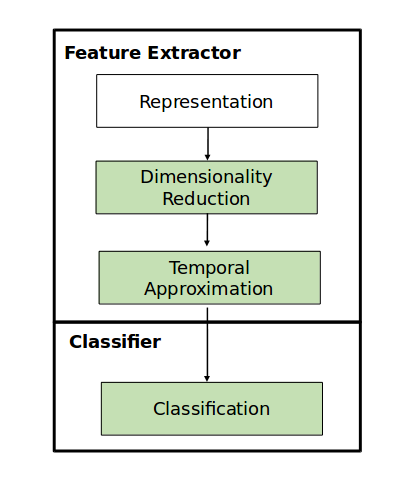
\includegraphics[width=0.4\textwidth]{fe1}
\caption{Error Back-propagation upto reduction operations }
 \label{fig:fe1}
 \end{figure}
\FloatBarrier

\noindent \textbf{Representation :} In \cite{choi_cnn} and \cite{EndToEnd}, CNN with log mel-power spectrogram as input was shown to be optimal for the music tagging task. Hence we compute the log-mel power spectrogram for all the analyses.\\
\\  
\textbf{Reduction :} The log mel power spectrogram is convolved with learnable filters. In \cite{MusicMotive}, 2D convolutions were shown to be more motivating than 1D. In \cite{choi_cnn}, a 5 layers of 2D convolutions were used for reduction, which achieves close to state of art performance on MTT dataset. Therefore, we choose their CNN model (algorithm \ref{alg:choicnn}) for dimensionality reduction.\\
\\  
\textbf{Temporal approximation :} Supervision can be introduced at this stage with a \textit{sequence to one} Recurrent Neural Network (see chapter 2 \ref{rnn}). Long Short-term memory(LSTM) and Gated recurrent units(GRU) are the choices at our disposal. In this thesis, we investigate only LSTMs. 
        
\subsection{Supervised learning of Temporal approximation and Classification operators}
\label{fe2}
The representation and reduction operators are not supervised on our target dataset. The representation and temporal approximation models are same as described in section \ref{fe1}. This model is also first trained on MTT dataset and then further fine-tuned on the target dataset. 
\begin{figure}[h] 
\centering
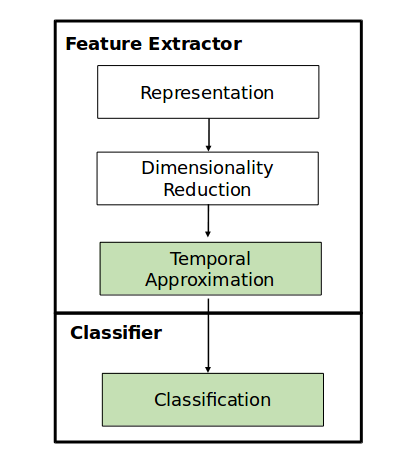
\includegraphics[width=0.4\textwidth]{fe2}
\caption{Error Back-propagation upto temporal approximation operations }
 \label{fig:fe2}
 \end{figure}
\FloatBarrier
\noindent \textbf{Reduction:} The CNN trained on large dataset is used as a black box feature extractor for the target classification task. That is, the weights converged on large dataset are not further modified by fine tuning on target dataset. In addition to black box CNN, we also investigate MFCCs because it is still not clear if CNNs can out perform MFCCs for a small dataset.

\subsection{Supervised learning only for Classification operators}
\label{fe3}
Supervision is not imposed on the feature extraction pipeline. The representation and reduction models are same as described in section \ref{fe2}
\begin{figure}[h] 
\centering
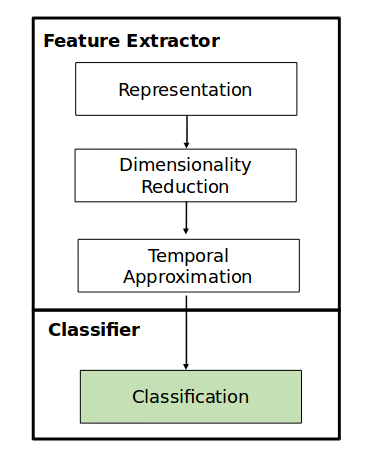
\includegraphics[width=0.4\textwidth]{fe3}
\caption{Error Back-propagation only through classifier }
 \label{fig:fe3}
 \end{figure}
\FloatBarrier 

\noindent \textbf{Temporal Approximation:} Bag of frames features (see Sec. \ref{clustering} ) obtained with unsupervised learning using K-means clustering algorithm was shown to be optimal for music tagging task in \cite{MultiScale}. Comparing Bag of frames features with RNN tells if deep learning with transfer learning can boost performance when training dataset is small. 